\usetikzlibrary{arrows.meta}

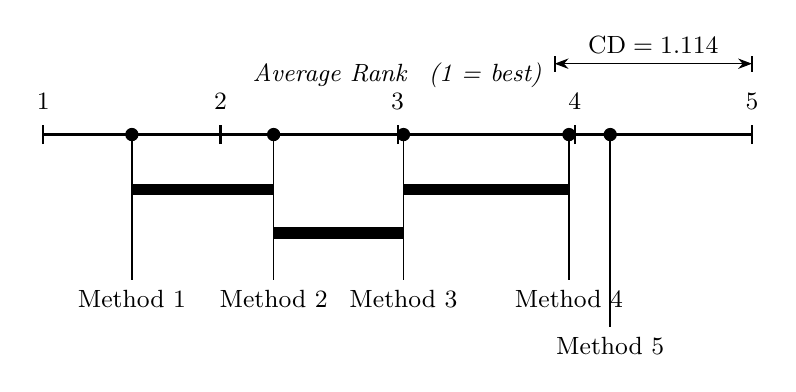
\begin{tikzpicture}[
  >=Stealth,
  font=\small,
  pin line/.style  = {draw=black, line width=0.6pt},
  sig bar/.style   = {draw=black, line width=4pt, line cap=butt},
  axis line/.style = {draw=black, line width=1.2pt},
  tick/.style      = {draw=black, line width=0.8pt},
]

% ── Coordinate system ──────────────────────────────────────────────────────
% Ranks 1..5 mapped linearly onto x = 0..9 cm
\def\axisW{9}
\def\kmax{5}
\pgfmathsetmacro{\scaleX}{\axisW / (\kmax - 1)}  % 2.25 cm per rank unit

\def\axisY{0}

% x positions of each method
\pgfmathsetmacro{\xA}{(1.500 - 1) * \scaleX}   % Method 1
\pgfmathsetmacro{\xB}{(2.300 - 1) * \scaleX}   % Method 2
\pgfmathsetmacro{\xC}{(3.033 - 1) * \scaleX}   % Method 3
\pgfmathsetmacro{\xD}{(3.967 - 1) * \scaleX}   % Method 4
\pgfmathsetmacro{\xE}{(4.200 - 1) * \scaleX}   % Method 5

% CD bracket half-width
\pgfmathsetmacro{\CDhalf}{1.1137 / 2 * \scaleX}

% ── Significance bars ──────────────────────────────────────────────────────
% Non-sig pairs (diff < CD = 1.1137):
%   Method 1--2 (diff=0.800), Method 2--3 (diff=0.733), Method 3--4 (diff=0.933)
%
% Bar slot assignment (bars hang below axis):
%   Bar 1 [M1--M2]: slot y = -0.7
%   Bar 2 [M2--M3]: overlaps Bar 1 horizontally -> slot y = -1.25
%   Bar 3 [M3--M4]: no overlap with Bar 1 -> slot y = -0.7

\def\barYone{-0.7}
\def\barYtwo{-1.25}

% Bar 1: Method 1 -- Method 2
\draw[sig bar] (\xA, \barYone) -- (\xB, \barYone);
% Bar 2: Method 2 -- Method 3
\draw[sig bar] (\xB, \barYtwo) -- (\xC, \barYtwo);
% Bar 3: Method 3 -- Method 4
\draw[sig bar] (\xC, \barYone) -- (\xD, \barYone);

% ── Label rows ─────────────────────────────────────────────────────────────
% Each method gets its own row, staggered to avoid overlap.
% Rows are assigned by inspecting x-distances: methods closer than ~1.8cm
% need to be on different rows.
%
% x positions (approx): M1=0.00, M2=2.92, M3=4.57, M4=6.68, M5=7.20
% M4 and M5 are only 0.52 cm apart -> different rows
% All others are >1.8 cm apart -> can share a row
%
% Row assignment (row 1 = highest, i.e. closest to axis):
%   Row 1 (y = -1.85): Method 1, Method 2, Method 3, Method 4
%   Row 2 (y = -2.45): Method 5

\def\rowOne{-1.85}
\def\rowTwo{-2.45}

% Pin bottom per method: reach below the lowest bar they belong to,
% then continue to their label row.
%   Method 1: Bar1 (y=-0.70) -> pin to row1
%   Method 2: Bar1+Bar2 (y=-1.25) -> pin to row1
%   Method 3: Bar2+Bar3 (y=-1.25) -> pin to row1
%   Method 4: Bar3 (y=-0.70) -> pin to row1
%   Method 5: no bar -> pin to row2

% Method 1
\filldraw[black] (\xA, \axisY) circle (2.2pt);
\draw[pin line]  (\xA, \axisY) -- (\xA, \rowOne);
\node[below, font=\small] at (\xA, \rowOne) {Method 1};

% Method 2
\filldraw[black] (\xB, \axisY) circle (2.2pt);
\draw[pin line]  (\xB, \axisY) -- (\xB, \rowOne);
\node[below, font=\small] at (\xB, \rowOne) {Method 2};

% Method 3
\filldraw[black] (\xC, \axisY) circle (2.2pt);
\draw[pin line]  (\xC, \axisY) -- (\xC, \rowOne);
\node[below, font=\small] at (\xC, \rowOne) {Method 3};

% Method 4
\filldraw[black] (\xD, \axisY) circle (2.2pt);
\draw[pin line]  (\xD, \axisY) -- (\xD, \rowOne);
\node[below, font=\small] at (\xD, \rowOne) {Method 4};

% Method 5  (bumped to row 2 to avoid overlap with Method 4)
\filldraw[black] (\xE, \axisY) circle (2.2pt);
\draw[pin line]  (\xE, \axisY) -- (\xE, \rowTwo);
\node[below, font=\small] at (\xE, \rowTwo) {Method 5};

% ── Rank axis ──────────────────────────────────────────────────────────────
\draw[axis line] (0, \axisY) -- (\axisW, \axisY);

\foreach \r in {1,...,5} {
  \pgfmathsetmacro{\tx}{(\r - 1) * \scaleX}
  \draw[tick] (\tx, \axisY-0.12) -- (\tx, \axisY+0.12);
  \node[above, yshift=2pt] at (\tx, \axisY+0.12) {\r};
}

\node[above, yshift=10pt] at (0.5*\axisW, \axisY+0.12)
  {\textit{Average Rank \enspace (1 = best)}};

% ── CD bracket ─────────────────────────────────────────────────────────────
\pgfmathsetmacro{\cdCX}{\axisW - \CDhalf}
\def\cdY{0.9}

\draw[{Stealth[length=5pt]}-{Stealth[length=5pt]}]
  (\cdCX-\CDhalf, \cdY) -- (\cdCX+\CDhalf, \cdY);
\draw[tick] (\cdCX-\CDhalf, \cdY-0.1) -- (\cdCX-\CDhalf, \cdY+0.1);
\draw[tick] (\cdCX+\CDhalf, \cdY-0.1) -- (\cdCX+\CDhalf, \cdY+0.1);
\node[above] at (\cdCX, \cdY) {$\mathrm{CD} = 1.114$};

% ── Caption ────────────────────────────────────────────────────────────────
% \node[below, align=center, font=\footnotesize] at (0.5*\axisW, \rowTwo-0.55)
  % {Connected methods are not significantly different
   % (Nemenyi, $\alpha=0.05$, $\chi^2_{F}=61.39$, $p=1.48\times10^{-12}$, $N=30$).};

\end{tikzpicture}
